\section{Προθεματική Αθροιστές}
Στην ενότητα αυτή θα παρουσιαστεί μια νέα υλοποίηση αθροιστών, οι αθροιστές προθέματος,
ο οποίοι έλαβαν σημαντικό ρόλο στην επιτάχυνση καθώς και μείωση του συνολικού εμβαδού 
των αθροιστών. 


\subsection{Πρόβλημα προθέματος}

Ένα prefix problem ή πρόβλημα προθέματος 
ορίζεται από n εξόδους y ( $y_{n-1},y_{n-2}, ... ,y_0 $ ) , n εισόδους x ( $x_{n-1},x_{n-1}, ... ,x_0 $ ) και τον τελεστή $\circledast$ .
Κάθε έξοδος y υπολογίζεται με τον παρακάτω τρόπο :
\begin{equation}
\begin{split}
y_0 &= x_0\\
y_1 &= x_1 \circledast x_0\\
y_2 &= x_2 \circledast x_1 \circledast x_0\\
&...\\
y_{n-1} &= x_{n-1} \circledast x_{n-2} \circledast ... \circledast x_{1} \circledast x_0\\
\end{split}
\end{equation}

Επίσης μπορούμε να το εκφράσουμε και αναδρομικά :
\begin{equation}
\begin{split}
y_0 &= x_0\\
y_{i} &= x_{i} \circledast y_{i-1}\\
\end{split}
\end{equation}

Ένα απλό παράδειγμα προβλημάτων που αντιμετωπίζονται ως προβλήματα προθέματος είναι 
η πρόσθεση πολλών αριθμών. Έστω πως έχουμε ένα σύνολο μεγέθους n από αριθμούς 
$(x_{n-1},x_{n-2}, ... ,x_1,x_0)$, σύμφωνα με τον ορισμό που δόθηκε παραπάνω
χρειαζόμαστε ένα ακόμα σύνολο ίδιου μεγέθους $(y_{n-1},y_{n-2}, ... ,y_1,y_0)$ 
όπου κάθε στοιχείο του συνόλου αυτού υπολογίζεται αναδρομικά
\begin{equation*}
\begin{split}
y_0 &= x_0\\
y_{i} &= x_{i} + y_{i-1}\\
\end{split}
\end{equation*}
και το τελικό αποτέλεσμα είναι καταχωρημένο στο $y_n-1$.

Το πρόβλημα υπολογισμού κρατουμένου μπορούμε να το μετατρέψουμε σε
prefix problem δημιουργώντας το ζεύγος $(G,P)$ και αναθέτοντας στον τελεστή
$\circledast$ την παρακάτω λειτουργιά :
\begin{equation}
\begin{split}
(g_i,p_i) \circledast (g_k,p_k) &= (g_i + p_ig_k , p_ip_k)\\
(G_i,P_i) \circledast (G_k,P_k) &= (G_i + P_iG_k , P_iP_k)
\end{split}
\end{equation}

Με αυτόν τον τρόπο μπορούμε να υπολογίσουμε κάθε ενδιάμεσο κρατούμενο $c_i$
καθώς και το κρατούμενο εξόδου $c_n$ για έναν αθροιστή των n-bits όπου $c_i = G_i$
και για $n \geq i \geq 0$ έχουμε 
\begin{equation}
\begin{split}
(G_0,P_0) &= (g_0,p_0)\\
(G_i,P_i) &= (g_i,p_i) \circledast (G_{i-1},P_{i-1})
\end{split}
\end{equation}
Η απόδειξη :
Εφόσον δεν υπάρχει κρατούμενο εισόδου ($c_{in} = c_{-1} = 0$) έχουμε 
\begin{equation*}
\begin{split}
    c_0 &= g_0 + p_0c_{-1} \\
    c_0 &= g_0 \\
    c_0 &= G_0
\end{split}
\end{equation*}
έστι το αποτέλεσμα ισχύει για $i-1$ \\
Αν $i>0$ και $c_{i-1} = G_{i-1}$ τοτε
\begin{equation*}
\begin{split} 
    (G_i,P_i)   &= (g_i,p_i) \circledast (G_{i-1},P_{i-1}) \\
                &= (g_i,p_i) \circledast (c_{i-1},P_{i-1}) \\
                &= (g_i + p_ic_{i-1} , p_iP_{i-1}) \\
            G_i &= g_i + p_ic_{i-1} \\
            G_i &= c_i
\end{split}
\end{equation*}
Επίσης ο τελεστής $\circledast$ έχει προσεταιριστική ιδιότητα 
\begin{equation*}
\begin{split} 
    (g_i,p_i)\circledast(g_j,p_j)\circledast(g_k,p_k) &= [g_i + p_ig_j,p_ip_j]\circledast(g_k,p_k) \\
    &= (g_i,p_i)\circledast[g_j + p_jg_k,p_jp_k]\\
    &= ( g_i + p_ig_j + p_ip_jg_k , p_ip_jp_k )
\end{split}
\end{equation*}

Παρακάτω παρουσιάζεται ένα γράφημα-δέντρο ( Εικόνα \ref{Serial-PrefixTree} ) 
ενός απλού διάδοσης κρατουμένου αθροιστή σε αναγόμενο σε πρόβλημα προθέματος.\\ 
\begin{figure}[H]
\centering
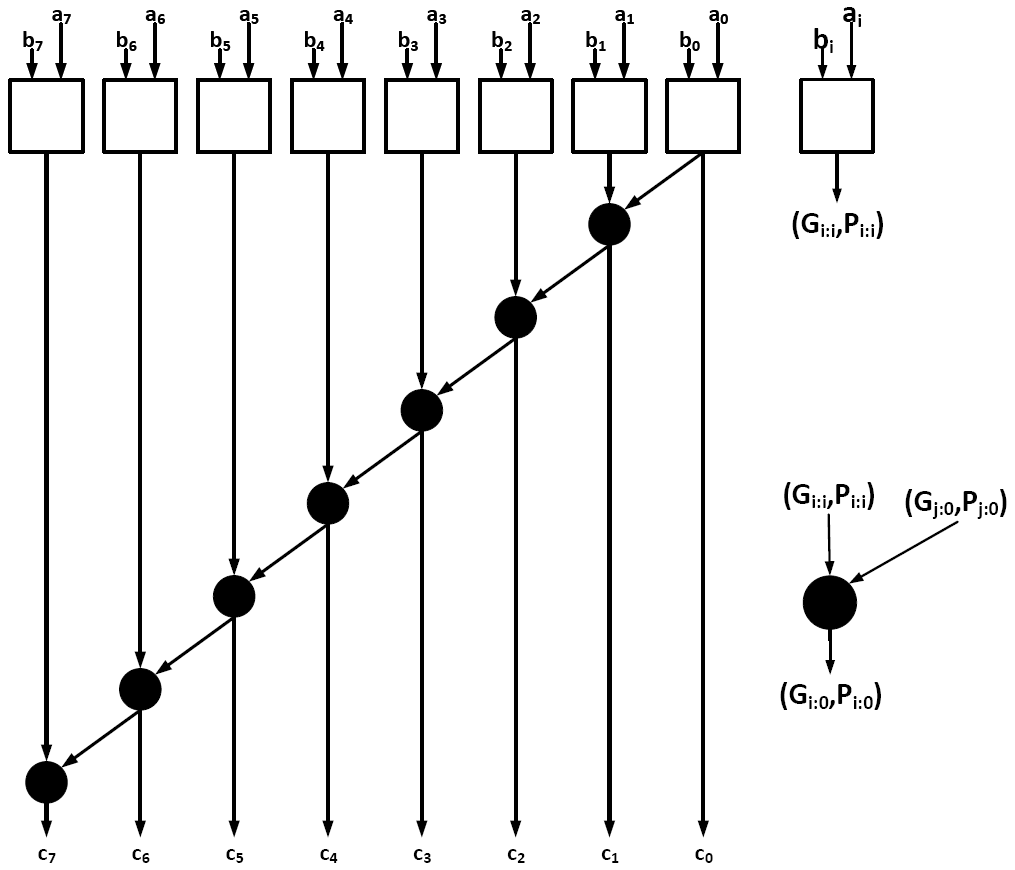
\includegraphics[scale=0.45]{Serial-Prefix.png}
\caption{Serial-Prefix Tree Adder}
\label{Serial-PrefixTree}
\end{figure}
Σε κάθε μαύρο κόμβο ουσιαστικά υλοποιείται η λογική συνάρτηση του τελεστή $\circledast$
που παρουσιάστηκε προηγουμένως. Ο παραπάνω αθροιστής υλοποιεί τον προθεματικό αλγόριθμο
σειριακά με αποτέλεσμα να είναι πολύ αργό το μοντέλο αλλά να καταλαμβάνει μικρότερο εμβαδόν
από άλλες τοπολογίες αθροιστών προθέματος που θα παρουσιαστούν στην συνέχεια.








\subsection{Παράλληλοι Προθεματικοί Αθροιστές}

\subsubsection{Brent-Kung Adder}

\subsubsection{Ladner-Fischer Adder}

\begin{figure}[H]
\centering
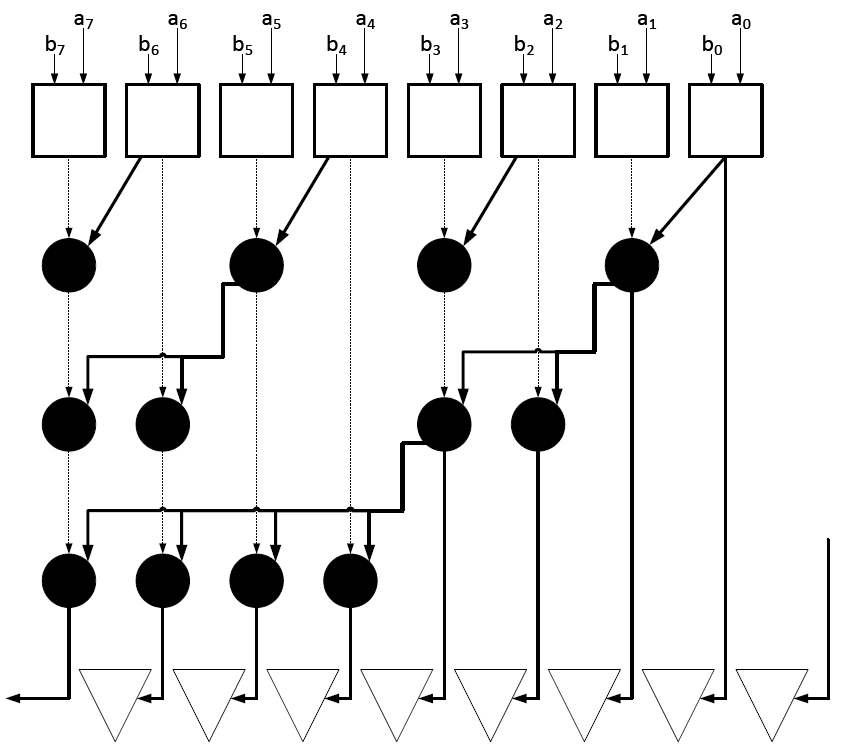
\includegraphics[scale=0.5]{Ladner-Fischer.png}
\caption{Ladner-Fischer Prefix Tree Adder}
\label{Ladner-FischerTree}
\end{figure}





\subsection{Δέντρα-Δομές Προθεμάτων}
